\documentclass[GA.tex]{subfiles}

\begin{document}


%\hyphenation{equi-va-len-cia}\hyphenation{pro-pie-dad}\hyphenation{res-pec-ti-va-men-te}\hyphenation{sub-es-pa-cio}

\chapter{Esquemas}

\section{Espectro y espacios localmente anillados}

\begin{defi}
Sea $A$ un anillo no trivial, es decir, que tiene ideales primos. Definimos $\mathrm{Spec}(A)$ como el conjunto de los ideales primos de $A$. 
\end{defi}

Por ejemplo, para $A=\Z$, $\mathrm{Spec}(\Z)=\{\{0\}\}\cup\{\Z_p\mid p$ primo$\}$. En este caso vemos que $\{0\}\subseteq\Z_p$ para todo $p$. 

Veamos ahora como ejemplo el caso $A=\C[x]$. En este caso, los ideales primos no nulos son los generados por polinomios irreducibles. Como $\C$ es algebraicamennte cerrado, son los de la forma $\gene{x-\alpha}$ con $\alpha\in\C$, así que podemos asociar este espectro a la recta afín compleja. De nuevo $\{0\}$ es primo y está contenido en todos los demás. 

Nótese que el ideal trivial solo es primo en dominios de integridad.

Dotamos a $\mathrm{Spec}(A)$ de una topología. Dado un ideal $I\subseteq A$, definimos $V(I)=\{\p\in\spec(A)\mid I\subseteq\p\}$. Se puede probar que $V(\sum_i I_i)=\bigcap_i V(I_i)$ y $V(I\cap J)=V(I)\cup V(J)$, $V(\{0\})=\spec(A)$ y $V(A)=\emptyset$, con lo que podemos definir la topología de Zariski sobre $\spec(A)$, que tiene como cerrados los conjuntos de la forma $V(I)$. Además se verifica que si $I\subseteq J$, entonces $V(J)\subseteq V(I)$. 

Si $f:A\to B$ es un homomorfismo de anillos, se define el functor contravariante $f^*:\spec(B)\to\spec(A)$ como $f^*(\p)=f^{-1}(\p)$ (el ideal contraído también denotado $\p^c$). Se comprueba fácilmente que $f^*$ es continua para la topología de Zariski y que cumple las propiedades para ser un functor contravariante. 

Vamos a definir \emph{el haz estructural en $\spec(A)$.} Para ello daremos varios pasos previos.

Denotamos $X=\spec(A)$ por simplicidad. Sea $f\in A$. Definimos $X_f=X\setminus V(\gene{f})=\{\p\in X\mid f\notin\p\}$. Sea $U\subseteq X$ un abierto, que por definición será de la forma $X\setminus V(I)$. Dado $\p\in U$, por definición $I\not\subseteq\p$, luego existe $f\in I$ con $f\notin\p$, así que $\p\in X_f\subseteq U$. Esto demuestra que los conjuntos $X_f$ forman una base de abiertos para $\spec(A)$. 

Recordemos que para $\p\in\spec(A)$, $S=A\setminus\p$ es un conjunto multiplicativamente cerrado (para más referencias consultar Atiyah-MacDonald, capítulo 3). Otro ejemplo importante de conjunto multiplicativamente cerrado es, para $f\in A$, el conjunto de las potencias de $f$, $\{1,f,f^2,\dots\}$. Es conveniente recordar también la definición del anillo localizado $S^{-1}A$ como el conjunto de pares $(a,s)\in A\times S$ de modo que $(a_1,s_1)\sim (a_2,s_2)$ si existe $t\in S$ tal que $t(a_1s_2-a_2s_1)=0$. Hay un homomorfismo evidente $h:A\to S^{-1}A$ dado por $h(a)=\frac{a}{1}$, que no es necesariamente inyectivo, pero verifica la siguiente propiedad universal: para todo anillo $B$ y para todo $\varphi:A\to B$ homomorfismo de anillos tal que $\varphi(s)$ es invertible para todo $s\in S$, existe un único homomorfismo $\psi$ que hace conmutar el siguiente diagrama
\[
\begin{tikzcd}
A\arrow[r, "h"]\arrow[dr, "\varphi"'] & S^{-1}A\arrow[d, dashed, "\exists!\psi"]\\
& B
\end{tikzcd}
\]

Se denota $A_\p$ al localizado de $A$ en $\p$, definido como $S^{-1}A$ para $S=A\setminus\p$. Se cumple que el ideal $\p A_\p$ es el ideal extendido de $\p$ por $h$. Este ideal está formado por las fracciones de la forma $\frac{a}{s}$ con $a\in\p$ y $s\notin\p$. Además este es el único ideal maximal, lo que convierte a $A_\p$ en un anillo local. 

\begin{ej}
En el anillo $\Z$ y con el ideal $\p=p\Z$, $\Z_\p=\{\frac{a}{s}\mid a\in\Z, p\not| s\}\subset\Q$. Se denota también $\Z_p$. Sea $p\Z_p=\gene{\frac{p}{1}}$. Sea $\frac{a}{s}\in\Z_p$ que no esté en el ideal. Entonces $s$ no es divisible por $p$, así que el inverso $\frac{s}{a}$ está bien definido. Entonces, todo elemento que no esté en el ideal es unidad, con lo que el ideal es maximal. 
\end{ej}

Ahora podemos definir el haz que pretendíamos, $$\OO_X(U):=\{s\in\prod_{\p\in U}A_\p\mid\forall\p\in U\exists a,f\in A: \p\in X_f\subseteq U\land s_\q=\frac{a}{f}\in A_\q \}.$$ Aquí $\prod$ denota el producto cartesiano y $s_\p$ denota los elementos de este producto cartesiano. La segunda propiedad de la definición nos garantizará que el haz está definido localmente y por lo tanto será realmente un haz. Concretamente, se están tomando fracciones que localmente tienen una expresión común. Se demuestra además que $\OO_X(U)$ es un subanillo de $\prod_{\p\in U}A_\p$. Las restricciones tienen la siguiente forma: dados $V\subseteq U$ podemos utilizar la proyección $\prod_{\p\in U}A_\p\to\prod_{\p\in V}A_\p$ (que es homomorfismo de anillos) para generar un homomorfismo de anillos $\OO_X(U)\to\OO_X(V)$. 

\begin{nota}
Si $X$ es un espacio topológico y tenemos definido para cada $x\in X$ un anillo o grupo abeliano (etc) $A_x$, se puede definir el prehaz $\calF(U)=\prod_{x\in U} A_x$ con las proyecciones como restricciones (que son todas sobreyectivas). Este prehaz es un haz. Obsérvese que la topología en particular que tenga $X$ no juega un papel relevante, así que se puede tomar la topología discreta. Una vez que tenemos definido este haz para la topología discreta podemos llevarlo a cualquier topología. Tenemos que la identidad $X^{dis}\to X$ es continua, donde $X^{dis}$ es $X$ con la topología discreta. Entonces, $Id_*\calF(U)=\calF(U)$ por definición. 
\end{nota}

Dado un anillo $A$, hemos construido un espacio topológico $\spec(A)$ al que le hemos asociado un haz de anillos $\OO_{\spec(A)}$. Al par $(\spec{A}, \OO_{\spec(A)})$ se le llama \emph{espectro} de $A$. 


\begin{ej}
Vimos que $X=\spec(\Z)$ se puede identificar con el conjunto de primos naturales unión el 0. Los cerrados de la topología de Zariski son, además del total (obtenido como $V(0)$) y del vacío, los de la forma $V(n\Z)$. Los ideales que contienen a $n\Z$ son los ideales generados por los divisores de $n$, luego los cerrados propios son los conjuntos finitos de primos. Como hemos visto, $\overline{0}=\spec(\Z)$. A esto lo llamaremos punto genérico. Los abiertos no triviales serían entonces el 0 y los conjuntos de primos con complementario finito. Denotamos $U_{p_1,\dots, p_r}$ al abierto que tiene como complementario el conjuto de primos indicado.  $U_\emptyset=X$. 

Vamos a calcuclar $\OO_X(U_{p})$. Tenemos que calcular $\Z_{\gene{p}}=\{\frac{a}{s}\mid a\in\Z, p\not| s\}$ y $\Z_{\gene{0}}=\Q$.  $U_{p}=X\setminus V(p\Z)=\{0\}\cup\{p_i\mid p\neq p_i\}$. Entonces $\OO_X(U_p)=\{(s_q)_{q\in U_p}\mid s_q\in\Z_{\gene{p}}\}=\Z_p=\{\frac{a}{p^r}\mid a\in\Z\}$ (esto habría que demostrarlo). 

Si cogemos un abierto genérico $U=U_{p_1,\dots, p_r}$, el resultado es $\OO_X(U)=\Z_{p_1\cdots p_r}$. En el caso del total, no ponemos ningún primo en el denominador, así que saldría simplemente $\Z$. La restricción $\OO_X(X)=\Z\to \OO_X(U)=\Z_{p_1\cdots p_r}$ es simplemente el homomorfismo usual de un anillo en el localizado. 
\end{ej}

\begin{ej}
Sea $k$ un cuerpo algebraicamente cerrado. $\spec(k[x])=k\cup\{\gene{0}\}$. La topología de zariski es análoga a la del anterior ejemplo, los abiertos no triviales son subconjuntos de $k$ con complementario finito en $k\cup\{0\}$. Si se hace el cálculo, se obtiene $\OO_{\spec(k[x)]}(k[x])=k[x]$. Si se toma un abierto que no sea el total, $\OO_{\spec(k[x])}(\{\alpha_1,\dots,\alpha_r\}^c)=k[x]_{(x-\alpha_1)\cdots(x-\alpha_r)}$. 
\end{ej}

\begin{prop}
Sea $A$ un anillo y $(\spec(A),\OO)$ su espectro.
\begin{enumerate}[(a)]
\item Para todo $\p\in\spec(A)$, la fibra $\OO_\p$ es isomorfa al anillo local $A_\p$.
\item Para todo elemento $f\in A$, si denotamos $X_f=\spec(A)\setminus V(\gene{f})$, entonces $\OO(X_f)$ es isomorfo al anillo localizado $A_f$.
\item En particular, $\OO(\spec(A))\cong A$. 
\end{enumerate} 
\end{prop}

\section{Esquemas}

En geometría diferencial se suelen definir las variedades diferenciables a partir de cartas en un atlas. Se pueden definir también de otro modo más próximo al que nos interesa en nuestro estudio. Dado $U\subseteq\R^n$ abierto, definimos el haz $E_U$ de funciones $C^{\infty}$, de modo que $\mathcal{E}_U(V)$ son las funciones $f:V\to\R$ de clase $C^{\infty}$ para $V\subseteq U$.

 Así que podríamos definir variedad diferenciable como un espacio topológico expresado como unión de abiertos $X=\cup X_i$ y un haz $E_X$ de modo que $(X_i,\mathcal{E}_X|_{X_i})\cong (U_i,\mathcal{E}_{U_i})$ con $U_i\subseteq\R^n$. Este isomorfismo es en el sentido de que hay un homeomorfismo entre los espacios topológicos y un isomorfismo de haces en el segundo elemento del par. Este enfoque será el que usemos para definir los esquemas. 
 
 
 \begin{defi}
 Un \emph{espacio anillado} es un par $(X,\calA)$ donde $X$ es un espacio topológico y $\calA$ es un haz de anillos (comutativos con unidad) en $X$.
 \end{defi}
 
 \begin{ejs}\
 \begin{enumerate}
 \item Sea $A$ un anillo fijo y $\calA$ el haz de todas las funciones con valor en $A$. 
 \item Dado un anillo topológico $A$ (por ejemplo $\R$ o $\C$), definimos $\calA$ como el haz de las funciones continuas con valores en $A$.
 \item Sea $X$ una variedad diferenciable (real) y $\calA$ el haz de las funciones $C^{\infty}$ con valores en $\R$.
 \item $(\spec(A), \OO_{\spec(A)})$. 
 \end{enumerate}
 
 \end{ejs}
 
 \begin{defi}
 Sean $(X,\calA)$, $(Y,\mathcal{B})$ espacios anillados. Un morfimo entre ellos es un par $(f, f^{\sharp})$ donde $f:X\to Y$ es continua y $f^{\sharp}:\mathcal{B}\to f_*\calA$ es un morfismo de haces de anillos en $Y$. 
 
\end{defi} 


\begin{ej}
Sean $X,Y$ variedades diferenciables y $f:X\to Y$ una aplicación diferenciable. Consideramos el haz de las funciones diferenciables $\mathcal{E}_X$ tal que $\mathcal{E}(U)$ es el anillo de funciones diferenciables de $U$ en $\R$, y hacemos lo mismo para $Y$. Recordemos que $(f_*\mathcal{E}_X)(V)=\mathcal{E}_X(f^{-1}(V))$. Por otro lado tenemos $\mathcal{E}_Y(V)$, pero dada $\varphi\in \mathcal{E}_Y(V)$, podemos asociarle $\varphi\circ f|_{f^{-1}(V)}\in\mathcal{E}_X(f^{-1}(V))$. Esta es la definición de $f^{\sharp}$. 
\end{ej}

Si tenemos tres haces $(X,\calA)\xrightarrow{(f,f^{\sharp})}(Y,\mathcal{B})\xrightarrow{(g,g^{\sharp})}(Z,\mathcal{C})$, tendríamos una composición $(g,g^{\sharp})\circ(f, f^{\sharp})$. La primera coordenada de la composición es simplemente $g\circ f$, pero en la segunda tenemos que hacerlo con más cuidado. Tenemos $f^{\sharp}:\mathcal{B}\to f_*\calA$, $g^{\sharp}:\mathcal{C}\to g_*\mathcal{B}$. Podemos considerar $g_*(f^{\sharp}):g_*\mathcal{B}\to g_*(f_*\mathcal{A})=(g\circ f)_*(\calA)$. Así que la segunda componente de la composición es $g_*(f^\sharp)\circ g^{\sharp}$. 



\begin{defi}
Un espacio anillado $(X,\calA)$ se dice \emph{localmente anillado} si para todo $x\in X$, la fibra $\calA_x$ es un anillo local.
\end{defi}


\begin{ej}
Sea $(X,\mathcal{E}_X)$ una variedad diferenciable, $x\in X$. Entonces $\mathcal{E}_{X.x}$ consideramos los gérmenes que se anulan en el punto $x$, que forman claramente un ideal. Si un germen no se anula en $x$, entonces tampoco se anula en un entorno, por lo que es invertible multiplicativamente, o sea, es una unidad en el anillo. Así que las variedades diferenciables son espacios localmente anillados.

Tenemos además un homomorfismo de anillos $v_x:\mathcal{E}_{X,x}\to \R$, que es la evaluación del gérmen en $x$. Se tiene que $\ker v_x=m$, ideal maximal por el primer teorema de isomorfía (el homomorfismo es sobreyectivo porque se puede tomar el gérmen constante). Este ideal es justamente el que hemos mencionado antes. Se demuestra que $m/m^2$ tiene la misma dimensión que la variedad diferenciable, y es lo que se llama espacio cotangente (el dual de él es el tangente). 
\end{ej}

\begin{defi}
Si $(A, \m)$ y $(B,\mathfrak{n})$ son anillos locales. Un homomorfismo $\varphi:A\to B$ se dice \emph{local} si $\varphi^{-1}(\mathfrak{n})=\m$. 
\end{defi}

\begin{defi}
Sean $(X,\calA), (Y,\mathcal{B})$ espacios localmente anillados. Diremos que un morfismo $(f,f^{\sharp}):(X,\calA)\to (Y,\mathcal{B})$ de espacios anillados es local cuando para cada punto $x\in X$, $f^{\sharp}_x:\mathcal{B}_{f(x)}\to\calA_x$ sea un homomorfismo local. 
\end{defi}

\begin{defi}
Un \emph{esquema afín} es un espacio localmente anillado $(X,\OO_X)$ que es isomorfo (como espacio localmente anillado) al espectro de algún anillo. Un \emph{esquema} es un espacio localmente anillado $(X,\OO_X)$ tal que $X$ se puede recubrir por abiertos $\{U_i\}_{i\in I}$ tales que $(U_i,\OO_X|_{U_i})$ es un esquema afín. 
\end{defi}


Vamos a ver que la correspondencia $A\to\spec(A)$ es functorial, y que además este functor es plenamente fiel. De hecho es equivalencia de categorías si nos restringimos a los esquemas afines, que son la imagen de este functor. 
\begin{prop}\label{inducido}
\begin{enumerate}[(a)]
\item Si $A$ es un anillo, $(\spec(A), \OO)$ es un espacio localmente anillado.
\item Si $\varphi:A\to B$ es un homomorfismo de anillos, $\varphi$ induce un morfismo natural de espacios localmente anillados
\[
\varphi^*=(f,f^\sharp):\spec(B)\to\spec(A)
\]
\item Si $A$ y $B$ son anillos, entonces cualquier morfismo de espacios localmente anillados $\spec(B)\to\spec(B)$ está inducido por un homomorfismo de anillos $A\to B$. 
\end{enumerate}
\end{prop}
\begin{dem}
Vamos a describir el morfismo $\varphi^*$. 

La aplicación $f:\spec(B)\to\spec(B)$ está definidad como $f(\p)=\varphi^{-1}(\p)$. Tenemos que probar que es continua, para lo cual, probaremos que $f^{-1}(V(I))=V(I^e)$, donde $I^e$ denota el ideal extendido. Si $\p\in f^{-1}(V(I))\Rightarrow f(\p)\in V(I)\Rightarrow \varphi^{-1}(\p)\supseteq I\Rightarrow \varphi^{-1}(\p)^e\supseteq I^e$. Como además $\p\in\varphi^{-1}(\p)^e$ (aunque no fuera primo), $\p\in V(I^e)$. Si ahora $\p\in V(I^e)$, $I^e\subseteq\p\Rightarrow I\subseteq \varphi^{-1}(I^e)\subseteq \varphi^{-1}(\p)$, luego $f(\p)=\varphi^{-1}(\p)\in V(I)$. Probar que $f$ es functorial para la composición es muy sencillo.

Definimos ahora $f^\sharp:\OO_{\spec(A)}\to f_*\OO_{\spec(B)}$. Consideramos la fibra $\OO_{\spec(A),\p}\cong A_{\p}$. Recordamos el ejercicio 1.8, que dice que $\Hom_X(f^{-1}\calF,\calG)\cong\Hom_Y(\calF, f_*\calG)$. Por esta propiedad podemos definir con más comodidad un morfismo $\tilde{f}^\sharp:f^{-1}\OO_{\spec(A)}\to \OO_{\spec(B)}$. Ahora las fibras que cogemos son, dado $\q\in\spec(B)$, $(f^{-1}\OO_{\spec(A)})_{\q}=\OO_{\spec(A), f(\q)}=\OO_{\spec(A), \varphi^{-1}(\q)}=A_{\varphi^{-1}(\q)}$. Por otro lado, $\OO_{\spec(B),\q}=B_{\q}$, por lo que basta definir un homomorfismo $A_{\varphi^{-1}(\q)}\to B_{\q}$ a partir de $\varphi:A\to B$. Por la propiedad universal de los anillos de fracciones, basta tomar la composición $A\to B\to B_{\q}$, tal que $a\in A\setminus\varphi^{-1}(\q)\mapsto\varphi(a)\in B\setminus\q\mapsto \frac{\varphi(a)}{1}$, que es una unidad. La propiedad universal nos que esta aplicación es única, y al precomponer con $A\to A_{\varphi^{-1}(\q)}$ el diagrama resultante es conmutativo. 
\[
\begin{tikzcd}
A\arrow[r,"\varphi"] \arrow[dr]\arrow[d] & B\arrow[d]\\
A_{\varphi^{-1}(\q)}\arrow[r, dashed, "\exists!"] & B_{\q}
\end{tikzcd}
\]
Faltaría probar que efectivamente el resultado es un morfimo de haces, lo cual se deja como ejercicio para el lector. 


\end{dem}

\begin{ej}[Fancy example of category equivalence]
Construimos la categoría $\CC'$ cuyos objetos son los números naturales y las flechas de $n\to m$ como las matrices $n\times m$ con coeficientes en $k$ (entendemos la matrices $n\times 0$ y $0\times m$ como un espacio de un punto. Hay una equivalencia de categorías evidente entre esta categoría y la de los $k$-espacios vectoriales de dimensión finito $\mathrm{Vec}_k$. Esto es, tenemos un functor $F:\CC\to\CC'$ que es esencialmente sobreyectivo: para todo $X\in Ob(\CC)$ existe $X'\in Ob(\CC)$ con $X\cong F(x')$; y además tiene que ser completamente fiel (fully faithful): esto es, que la aplicación $F_{X,Y}: \Hom(X,Y)\to \Hom(FX,FY)$ entre los conjuntos de homomorfismos es biyectiva para cada par de objetos $X$ e $Y$. Si el functor fuera contravariante, se ajustaría de manera evidente la definición.

También se puede definir en términos de la existencia un functor ``inverso''. 
\end{ej}

\begin{ejs}[Ejemplos de $\spec$]\
\begin{enumerate}
\item Sea $k$ un cuerpo.  $\spec(k)=(\{\{0\}\}, k)$. 
\item \emph{Anillos de valuación discreta (DVR)}.  Antes de dar la definición damos un ejemplo. Consideramos $\Z_p$, de modo que $\spec(\Z_p)=\{\{0\}, p\Z_p\}$, con $p\Z_p$ como único punto cerrado. Un anillo de valoración discreto es un dominio de integridad local que es dominio de ideales principales. $\Z_p\setminus\{0\}=\{\frac{m}{n}\mid m,n\in\Z, p\not| n\}$. Definimos $v_p:\Z_p\setminus\{0\}\to\N$ como $v_p(\frac{m}{n})=\max\{e\geq 0\mid p^e|m\}$, que es lo que se llama una valuación discreta. En todo anillo de evaluación discreta $A$, $\spec(A)$ es homeomorfo al caso $\Z_p$, es decir, de la forma $\{\{0\},\m\}$. En este caso
\[
\OO_{\spec(A)}(U)=\begin{cases}
\{0\} & U=\emptyset\\
Q(A) & U=\{\{0\}\}\\
A & U=\spec(A)
\end{cases}
\]
donde $Q(A)$ es el cuerpo de fracciones. 
\end{enumerate}
\end{ejs}

\begin{ej}
Para el cuerpo $\R$, se puede definir el espacio afín $\R^n$ con la topología de Zariski. Para $n=1$, el anillo de funciones regulares sería $k[x]$. Desde el punto de vista de teoría de esquemas, se define el espacio afín de dimensión uno como $\A_{\R}^1=\spec(\R[x])$, que vamos a ver que contiene mucha más información. Para comprobarlo, vemos los ideales primos de $\R[x]$, que son $\{0\}$ (punto denso), los ideales de la forma $\gene{x-\alpha}$ (que son los que están en correspondencia biunívoca con $\R$), y todos los demás ideales generados por un polinomio mónico irreducible (que son de la forma $x^2-2\alpha x+(\alpha^2+\beta^2)$ con $\alpha,\beta\in\R$, $\beta\neq 0$, es decir, que tenga como raíces $\alpha\pm\beta i$). Como conjunto, tenemos un punto especial, el conjunto $\R$ y los números complejos cocientados por la relación del conjugado. Los abiertos serían simplemente el complementario de un conjunto finito de puntos elegidos de $\R$ y el conjunto cociente de $\C$. 
\end{ej}

\begin{ej}[Pegamiento de esquemas]
Para pegar esquemas primero tenemos que saber cómo se pegan haces (se puede ver también en el ejercicio 1.22). Sea $X$ un espacio topológico y $\bigcup_{i\in I}U_i$ un recubrimiento abierto. Sea $\calF_i$ un haz en $U_i$ con las siguientes propiedades:
\begin{enumerate}
 \item
  Para cada para $(i,j)$, existe un isomorfismo $\varphi_{ij}:\calF_i|_{U_i\cap U_j}\to\calF_j|_{U_i\cap U_j}$. 
 \item $\varphi_{ii}=Id_{\calF_i}$.
 \item Denotando $U_{ijk}=U_i\cap U_j\cap U_k$, $\varphi_{jk}|_{U_{ijk}}\circ\varphi_{ij}|_{U_{ijk}}=\varphi_{ik}|_{U_{ikj}}$
 \end{enumerate}
 Entonces existe un haz $\calF$ en $X$ y existe un isomorfismo $\psi_i:\calF|_{U_i}\to\calF_i$ tal que conmuta
 \[
 \begin{tikzcd}
 \calF|_{U_{ij}}\arrow[r, "\psi_i|_{U_{ij}}"]\arrow[d, "\psi_j|_{U_{ij}}"'] &\calF_i|_{U_{ij}}\arrow[dl, "\varphi_{ij}"] \\
 \calF_j|_{U_{ij}} &
 \end{tikzcd}
 \]
 Este par es único salvo isomorfismo único.
 
 Vamos ahora al pegamiento de esquemas. Sean $X_1, X_2$ esquemas. Sean $U_i\subseteq X_i$ abiertos y sea $\varphi:(U_1,\OO_{X_1}|_{U_1})\to(U_2,\OO_{X_2}|_{U_2})$ un isomorfismo. 
 
\begin{lemma}
Si $X=\spec(A)$, todo abierto de $X$ es un esquema.
\end{lemma}
\begin{proof}
Sea $U\subseteq X$ abiertos. Dado $f\in A$, sabemos que los abiertos $X_f$ son una base de abiertos, luego $U=\cup X_{f_i}$. Tenemos $(U,\OO_X|_U)$, que a su vez restringe a $(X_{f_i}, \OO_X|_{X_{f_i}})$, que se puede ver que es isomorfo a $\spec(A_{f_i})$ usando resultados de álgebra conmutativa y la construcción hecha hasta ahora. Gracias a esto $\varphi$ es un isomorfismo de esquemas. Entonces existe un esquema $\widetilde{X}=\widetilde{X}_1\cup\widetilde{X}_2$, donde los subespacios escritos son abiertos del total, tal que $(\widetilde{X}_i,\OO_{\widetilde{X}_i}\cong(X_i,\OO_{X_i})$ mediante $\psi_i$. Este espacio cumple que $\psi_1^{-1}(U_1)=\psi^{-1}_2(U_2)$ en $X$ y además $\varphi\circ\psi_1|_V=\psi_2|_V$. Este espacio es el espacio de pegamiento usual en topología. 
\end{proof}
\end{ej}

\begin{ej}
$\spec(k[x]/\gene{x^2})=\{\gene{\overline{x}}\}$, ya que los primos de este anillo son los primos de $k[x]$ que contienen a $\gene{x^2}$, que solo hay uno.  Como espacio anillado tiene el haz que a cualquier abierto no vacío le asigna $k[x]/\gene{x^2}$, lo cual se puede ver notando que este anillo es de la forma $k[\varepsilon]=\{a+b\varepsilon\mid a,b\in k, \varepsilon^2=0\}$.
\end{ej}

\begin{ej}
Sea $(X,\mathcal{E})$ una variedad diferenciable y $\alpha:\spec(\R)=(\{*\},\R)\to (X,\mathcal{E})$ morfismo de espacios localmente anillados sobre $\R$ (es decir, de $\R$-álgebras). Necesariamente $\alpha(*)=p\in X$. $\alpha^{\sharp}:\mathcal{E}\to\alpha_*\R$, donde $\alpha_*\R(U)=\R(\alpha^{-1}(U))=0$ si $p\notin U$ y $\R$ en caso contrario. Para $p\in U$ tenemos
\[
\begin{tikzcd}
\mathcal{E}(U)\arrow[r, "\alpha^{\sharp}(U)"]\arrow[r, "\alpha^{\sharp}(U)"]\arrow[d]& \R\arrow[d, equals]\\
\mathcal{E}_p\arrow[r, "\alpha^{\sharp}_p"]\arrow[r] & \R
\end{tikzcd}
\]
Dado $\zeta\in \mathcal{E}(U)$ y su germen $\zeta(p)=c$, $\zeta=(\zeta-c)+c$, luego $\zeta_p=(\zeta_p-c)+c$, estando el término entre paréntesis en el ideal maximal $\m_p$ (los gérmenes que se anulan en $p$), luego $\alpha^{\sharp}(\zeta_p)=c$ por ser homomorfismo de $\R$-álgebras. 
\end{ej}

\begin{ej}
Siguiendo el ejemplo anterior, tomamos ahora $\alpha:\spec(\R[\varepsilon])\to (X,\mathcal{E})$. De nuevo $\alpha:\{*\}\to X$ tiene imagen $p\in X$ y $\alpha_*(\R[\varepsilon])$ es $\R[\varepsilon]$ si $p\in U$ y 0 en otro caso. También $\alpha^{\sharp}(U)$ será un homomorfismo de $\R$-álgebras local. 
\[
\begin{tikzcd}
\mathcal{E}(U)\arrow[r] \arrow[d] &\R[\varepsilon]\\
\R[\varepsilon]\arrow[ur, "\alpha^{\sharp}_p=\beta"]&
\end{tikzcd}
\]
Como $\beta$ es local, $\beta(\m_p)\subseteq\gene{\varepsilon}$ y $\beta(\m^2_p)\subseteq\gene{\varepsilon}^2=\{0\}$. Por otra parte tenemos la evaluación $ev_p:\mathcal{E}\to \R$ y $\pi:\R[\varepsilon]\to \R=\R[\varepsilon]/\gene{\varepsilon}$. Así que $\beta(\m_p)\subseteq\ker\pi$. Se tiene en realidad que $\ker\pi=\R\varepsilon$, puesto que $\R[\varepsilon]=\R\oplus\R\varepsilon$. Podemos definir entonces $\overline{\beta}:\m_p/\m^2_p\to\R\varepsilon$ que es $\R$ lineal, es decir, es un vector tangente. 
\end{ej}

\begin{ej}
Si $k$ es un cuerpo algebraicamente cerrado, podíamos considerar el espacio afín $k^n$ con la topología de Zariski. Desde el punto de vista esquemático, si tomamos $A=k[x_1,\dots, x_n]=k[x]$, $\spec(A)=\A_k^n=(\spec(k[x]),\OO_{\A_k^n})$. Hay una relación entre estas dos construcciones. Cada punto de $k^n$ nos da un ideal maximal, luego $\tau:k^n\hookrightarrow\spec(k[x])$ mediante $a\mapsto \gene{x_1-a_1, \dots, x_n-a_n}$. Entonces $\Ima\tau$ se llama espectro maximal de $k[x]$. Además $\tau$ es na inmersión topológica (es homeomorfismo sobre su imagen). Dado un ideal cualquiera $I\subseteq k[x]$ y consideramos $\tau^{-1}(V(I))=\{a\in k^n\mid \tau(a)\supseteq I\}=\{a\mid I\supseteq \gene{x_1-a_1, \dots, x_n-a_n}=\{a\mid f(a)=0, \forall f\in I\}=V(I)$ (abusamos de notación, el primer $V(I)$ es el del espectro y el segundo el de la geometría algebraica clásica). Se comprueba además que $\tau^{-1}\OO_{\A_k^n}$ es el haz de las funciones regulares en $k^n$. 
\end{ej}

Lo siguiente será construir el proyectivo en versión esquemática. Sea $S=\bigoplus_{d=0}^{\infty}S_d$ un anillo graduado (recordemos que la suma es como grupos aditivos, $1\in S_0$, Y $S_dS_e\in S_{d+e}$). Clásico ejemplo el de los polinomios en varias variables con grado la suma de los exponentes de las variables. Los elementos de $S_d$ se llaman homogéneos. Denotamos $S_+$ como la suma directa cuando $d>0$ (denominado ideal irrelevante por analogía al ejemplo mencionado). 

\begin{defi}
Un ideal $I\subseteq S$ se dice \emph{homogéneo} cuando $I=\bigoplus_{d=0}^{\infty}(I\cap S_d)$, lo cual es equivalente a decir que $I$ está generado por elementos homogéneos. Recordamos que en estas condiciones $S/I=\bigoplus_{d=0}^{\infty}S_d/(I\cap S_d)$.
\end{defi} 

Dado un anillo graduado $S$, definimos $\proj(S)=\{\p\in\spec(S)\mid \p$ homogéneo, $\p\not\supseteq S_+\}$. Definismos sobre este conjunto la topología cuyos cerrados son de la siguiente forma: si $I$ es un ideal homogéneo, definimos $V(I)=\{\p\in\proj(S)\mid \p\supseteq I\}$. Por ejemplo, $V(S_+)=\emptyset$ y $V(\{0\})=\proj(S)$. Por el lema 2.4 de Hartshore se verifican las propiedades necesarias para que estos conjuntos sean los cerrados de una topología, a la que llamamos topología de Zariski. A veces, para distinguirla de la topología de $\spec(S)$, escribiremos $V^h$ en lugar de $V$.

Obsérvese que $\proj(S)\subset\spec(S)$. De hecho, se tiene que $\proj(S)$ tiene la topología inducida por $\spec(S)$\footnote{\href{https://math.stackexchange.com/questions/2747367/is-the-zariski-topology-of-proj-s-the-same-as-the-subspace-topology-of-spec-s}{Prueba}}.

Definimos ahora un haz de anillos $\OO_{\proj(S)}$. Para ello vamos a definir primero $S_{(\p)}$ para $\p\in\proj(S)$. Sea $T\subseteq S\setminus\p$ el conjunto multiplicativo de todos los elementos homogéneos de $S$ que no están en $\p$. Escrito de otra forma $T=\bigcup_{d=0}^{\infty}(S\setminus\p)\cap S_d$. Entonces $S_{(\p)}$ son los elementos de grado 0 de $T^{-1}S=\{\frac{s}{t}\mid s\in S, t\in T\}$, esto es que $s$ y $t$ sean homogéneos del mismo grado.

\begin{ej}
Sea $S=\Z[x_1,\dots, x_n]$, $n\geq 2$. Tomamos $\p=\gene{x_1}$, que es ideal primo (el cociente sale dominio de integridad) homogéneo (generado por un polinomio homogéneo) que no contiene al ideal irrelevante. Otro ejemplo más interesante es $\q=\gene{x_1^3+x_2^3+x_3^3}$ para $n=3$. Se demuestra que el polinomio que lo genera es irreducible en $\Z$ y por tanto es primo. Como $\q$ no contiene a ninguna de las variables, no contiene al irrelevante. Llámamos $V_c(\q)=\{(a_1, a_2,a_3)\in\Z^3\mid a_1^3+a_2^3+a_3^3=0\}$ ($c$ de clásico). Por el teorema de Fermat sabemos que alguno de los $a_i$ tiene que ser 0, luego es fácil encontrar las soluciones enteras de esta ecuación. Si consideramos en lugar de este $V_c$, el $V$ en $\proj(S/\q)$ recuperaremos la información de esta ecuación y mucha más, además de poder encontrarla sobre otros anillos. Como en general no sabemos dónde es mejor buscar las soluciones, es preferible el enfoque esquemático. 
\end{ej} 

Finalmente, $\OO_{\proj(S)}(U)=\{s=(s_{\p})_{\p\in U}\mid s_{\p}\in S_{(\p)}, \forall \p\in U\exists V\ni\p,V\subseteq U, \exists a,f\in S$ homogéneos del mismo grado de modo que $\forall\q\in V, f\notin\q, s_{\q}=\frac{a}{f}\in S_{(\q)}\}\subset\prod_{\p\in U} S_{(\p)}$. Se comprueba que esto efectivamente da un haz.  

\begin{prop}
En las condiciones anteriores
\begin{enumerate}[(a)]
\item $\forall\p\in\proj(S)$, $\OO_{\proj(S),\p}=S_{(\p)}$ como anillo local (habría que probar primero que $S_{(\p)}$ es local).
\item Para $f\in S_+$ homogéneo, $D_+(f)=\{\p\in\proj(S)\mid f\notin\p\}$ es una base de abiertos. Además, $(D_+(f),\OO|_{D_+(f)})\cong\spec(S_{(f)})$ como espacio localmente anillado, donde $S_{(f)}$ es el conjunto de fracciones que en el denominador tiene una potencia de $f$ y el numerador tiene el mismo grado que esta potencia.
\item Como corolario, obtenemos que $\proj(S)$ es un esquema. 
\end{enumerate}
\end{prop}

\begin{ej}
Sea $S=A[x_0,\dots, x_n]$ con $A$ un anillo cualquiera. Entonces denotamos $\proj(S)=\PP^n_A$ y lo denominamos \emph{espacio proyectivo} $n$-dimensional sobre $A$. En el caso particular de que $A$ sea un cuerpo, entonces el espacio proyectivo es un esquema cuyo subespacio de puntos cerrados es homeomorfo a la variedad algebraica llamada espacio proyectivo $n$-dimensional. 
\end{ej}

\section{Categorías}
\subsection{Productos y coproductos}

\begin{nota}[Lenguaje categórico]
Una subcategoría se dice \emph{plena} (full subcategory) si los morfismos en la subcategoría son todos los que había en la categoría inicial entre los objetos de la subcategoría. Por ejemplo, la categoría de haces es una subcategoría plena de la categoría de prehaces, pero la categoría de espacios localmente anillados no es una subcategoría plena de la categoría de espacios anillados.
\end{nota}

\begin{defi}
Sea $\CC$ una categoría. Dados dos objetos $X,Y$ de $\CC$, un \emph{producto} de $X$ e $Y$ es una tripleta $(Z,p,q)$ donde $Z$ es un objeto de $\CC$, $p:Z\to X$ y $q:Z\to Y$ verificando la siguiente propiedad universal: para todo $U\in Ob(\CC)$ y para todo $\alpha:U\to X, \beta:U\to Y$, existe un único $\gamma:U\to Z$ tal que $p\circ\gamma=\alpha$ y $q\circ\gamma=\beta$, o dicho con un diagrama conmutativo
\[
\begin{tikzcd}
& U\arrow[dl, "\alpha"]\arrow[dr, "\beta"]\arrow[d, dashed, "\exists!\gamma"] & \\
X & Z\arrow[r, "q"]\arrow[l, "p"] & Y
\end{tikzcd}
\]
\end{defi}
Es fácil probar que, en caso de existir, este objeto es único salvo isomorfismo único.
\begin{ej}
Para $\CC=\mathrm{Set}$, el producto es el producto cartesiano con las proyecciones. Para $\CC=\mathrm{Vec}_k$ también tenemos el producto cartesiano usual. Lo mismo con $\CC=\mathrm{Top}$. 
\end{ej}

\begin{defi}
Un \emph{coproducto} de $X$ e $Y$ es un producto en $\CC^{op}$. 
\end{defi}
\begin{defi}
En $\mathrm{Set}$ y $\mathrm{Top}$ el coproducto es la unión disjunta. Mientras que en $\mathrm{Vec}_k$ es la suma directa (que es lo mismo que el producto cartesiano), así que el producto y el coproducto de espacios vectoriales son isomorfos (esto pasa también es los $R$-módulos y cualquier otra categoría abeliana). 
\end{defi}

Vamos a centrarnos ahora en la categoría $\mathrm{Ring}$. Aquí el producto no es más que el producto cartesiano. El coproducto sin embargo es $A\otimes_{\Z} B$. Aquí el producto está definido como $(a\otimes b)(a'\otimes b')=(aa')\otimes (bb')$. La propiedad universal se cumple para $a\mapsto a\otimes 1$ y $b\mapsto 1\otimes b$ (el elemento neutro es $1\otimes 1$). 

\begin{defi}
Un objeto $F$ es \emph{final} en $\CC$ si para todo objeto $X$ existe un único morfismo $X\to F$. Un objeto $I$ es \emph{inicial} si es final en la categoría opuesta.
\end{defi}
Dos objetos finales son siempre isomorfos mediante isomorfismo único.

\begin{ej}
En $\mathrm{Set}$ un objeto final es $\{*\}$ y el objeto inicial es $\emptyset$. Igual en $\mathrm{Top}$. En $\mathrm{Vec}_k$ el final y el inicial es el espacio vectorial trivial. En $\mathrm{Ring}$ el objeto final es el anillo nulo. El objeto inicial es $\Z$ porque el único morfismo es $1\mapsto 1_R$. 
\end{ej}

Las categorías en las que $I\cong F$, este objeto se denomina objeto nulo. 

Nuestro objetivo a partir de ahora será probar que en la categoría de esquemas $\mathrm{Sch}$ existen productos. Por el ejercicio 2.4, tenemos que
\[
\Hom_{\mathrm{Sch}}(X,\spec(A))\cong\Hom_{\mathrm{Ring}}(A,\OO_x(X)).
\]

El isomorfismo es una biyección de conjuntos. Obsérvese la similitud de este resultado con el del ejercicio 1.18, es decir
\[
\Hom_{\mathrm{Sh}_X}(f^{-1}\calG,\calF)\cong \Hom_{\mathrm{Sh}_Y}(\calG, f_*\calF)
\] 

que nos daba una adjunción de functores. En el caso de los esquemas, tenemos un functor $\spec:\mathrm{Ring}\to \mathrm{Sch}$. En sentido opuesto tenemos el functor $(X,\OO_X)\mapsto \OO_X(X)$. Vamos a tratar más en detalle el fuctor $\spec$. A nivel de objetos tenemos claro cómo funciona. A nivel de morfismos la proposición 2.3 de Hartshorne nos da el funcionamiento, que como se observa es contravariante. Por ser contravariante, para que las dos ecuaciones sean totalmente análogas habría que poner la categoría opuesta en $\mathrm{Ring}$ o $\mathrm{Sch}$, ya que sin eso los objetos están ``en orden contrario''. Vamos a ver en detalle quién es el morfismo de espacios anillados. Si llamamos $f:\spec(B)\to\spec(A)$ al morfismo inducido por $\varphi:A\to B$, buscamos un morfismo $\OO_{\spec(A)}\to f_*\OO_{\spec(B)}$, o por el ejercicio 2.4, $f^{-1}\OO_{\spec(A)}\to \OO_{\spec(B)}$. Se tiene que $(f^{-1}\OO_{\spec(A)})_q=\OO_{\spec(A),f(q)}\cong A_{q^c}$ y por otro lado $(\OO_{\spec(B)})_q\cong B_q$. El morfismo que buscamos es el que hace conmutar el diagrama
\[
\begin{tikzcd}
A\arrow[r, "f"]\arrow[d] & B\arrow[d]\\
A_{q^c}\arrow[r, dashed] & B_q
\end{tikzcd}
\]
Como este homomorfismo es local, se tiene de hecho un morfismo de espacios localmente anillados. 


Ahora nos interesa buscar objetos iniciales y finales en la categoría de los esquemas. Vamos a ver que el objeto final es $\spec(\Z)$. Esto se tiene del ejercicio 2.4 por ser $\Z$ objeto inicial de los anillos. Del mismo modo podemos obtenemos el objeto inicial. 
\
\begin{observacion}
$\spec(\{0\})=(\emptyset,\{0\})$, ya que un ideal primo por definición no puede ser el total. 
\end{observacion}

\begin{defi}
Sea $S$ un esquema. Un esquema sobre $S$ es una flecha de esquemas $X\to S$. Un morfismo de esquemas sobre $S$ es un morfismo de esquemas $X\to Y$ que conmute con las flechas hacia $S$. 
\end{defi}

Esta construcción es general en cualquier categoría, y es lo que se llama la categoría \emph{slice}. 


Sea $\CC$ una categoría y $X,Y\in Ob(\CC)$. Sea un functor $F=F_{X,Y}:\CC\to\mathrm{Set}$ definido en los objetos como $F(U)=\Hom_{\CC}(U,X)\times\Hom_{\CC}(U,Y)$ y en los morfismos $F(\alpha):F(U')\to F(U)$ es contravariante, definido como $F(\alpha)(f,g)=(f\circ \alpha, g\circ\alpha)$. Dado $Z\in Ob(\CC)$ definimos $h_z:\CC\to\mathrm{Set}$ como el archiconocido functor $h_Z=\Hom_{\CC}(-,Z)$. Recordamos que este functor actúa en los morfismos como $h_Z(\alpha):\Hom(B,Z)\to \Hom(A,Z); h_Z(\alpha)(\beta)=\beta\circ\alpha$, donde $\alpha:A\to B$. 

\begin{defi}
Un functor contravariante $G:\CC\to\mathrm{Set}$ se dice \emph{representable} si $\exists Z\in Ob(\CC)$ y $\exists\gamma$ transformación natural entre $G$ y $h_Z$. Vamos a definir ahora lo que significa una transformación natural (morfismo en la categoría de los functores) $\tau:G\to H$ entre dos functores $G,H:\CC\to\CC'$ (que vamos a suponer covariantes para escribir la definición) es una familia $\tau(U):G(U)\to H(U)$ haciendo conmutar el diagrama
\[
\begin{tikzcd}
G(U)\arrow[r, "\tau(U)"]\arrow[d, "G(\alpha)"'] & H(U)\arrow[d, "H(\alpha)"]\\
G(U')\arrow[r, "\tau(U')"] & H(U')
\end{tikzcd}
\]
Se comprueba en seguida que las transformaciones naturales se pueden componer y que existe la transformación natural identidad de un functor en sí mismo. Llamaremos isomorfismo de functores a $\tau:G\to H$ cuando $\tau(U)$ es isomorfismo para todo objeto $U\in Ob(\CC)$, que es equivalente a que tenga un inverso a los dos lados. 
\end{defi}

\begin{prop}
$(Z,p,q)$ es un producto de $X,Y$ si y solo si $h_Z\cong F_{X,Y}$. 
\end{prop}
\begin{dem}
Sea $(Z,p,q)$ un producto. Entonces, para todo $\alpha:U\to X$, $\beta:U\to Y$ existe un único $\gamma:U\to Z$ tal que $q\gamma=\beta$ y $p\gamma=\alpha$. A cada $\gamma\in\Hom_{\CC}(U,Z)$ le asociamos $(p\gamma,q\gamma)\in F_{X,Y}(U)$. La propiedad universal del producto implica que esto es un isomorfismo. Recíprocamente, supongamos que existe un isomorfismo $\tau:h_Z\to F_{X,Y}$. El objeto del producto será $Z$. Tenemos que $\tau(Z):h_Z(Z)\to F_{X,Y}(Z)$, por lo que tomamos $(p,q)=\tau_Z(Z)(Id_Z)=(p,q)$, que verificará la propiedad universal del producto por ser $\tau$ isomorfismo. 
\end{dem}

Denotamos como $h_{\alpha}$ para $\alpha:X\to X'$ a la transformación natural $h_{\alpha}:h_X\to h_{X'}$ dado por $h_{\alpha}(U)(g)=\alpha\circ g$

\begin{lemma}[de Yoneda]
$h_*:\CC\to \mathrm{Fun}(\CC, \mathrm{Set})$ es plenamente fiel, es decir, para todo $X,X'\in Ob(\CC)$ la aplicación $\alpha\in\Hom_{\CC}(X,X')\mapsto h_{\alpha}$ es un isomorfismo. 
\end{lemma}
La demostración se deja como ejercicio. 

Como consecuencia, $X,Y$ tiene un producto $Z$ en $\CC$ si y solo si $h_Z\cong h_X\times h_Y$ definido como $(h_X\times h_Y)(U)=h_X(U)\times h_Y(U)$. De igual modo con el coproducto. 

\subsection{Categorías aditivas y abelianas}
Sea $\CC$ una categoría cumpliendo que $\Hom_{\CC}(X,Y)$ es un grupo abeliano (no con la composición) y existen productos y coproductos finitos. A esto lo llamaremos categoría aditiva. Por el lema de Yoneda $h_{X\times Y}\cong h_X\times h_Y$, aunque en este caso $h_*:\CC\to\mathrm{Fun}(\CC, \mathfrak{Ab})$. Como en grupos abelianos el producto y el coproducto son isomorfos (la suma directa), en cualquier categoría aditiva también, puesto que $h_{X\oplus Y}\cong h_X\oplus h_Y$. Vamos a añadir un axioma que en realidad se puede probar a partir de los existentes considerando el producto y coproducto de familias vacías, que es que toda categoría aditiva debe contener un objeto nulo. 

\begin{ej}
La categoría $\mathfrak{Ab}$ es aditiva. Si $R$ es un anillo conmutativo, $\mathrm{Mod}_R$ es aditiva. Los espacios vectoriales normados (bajo la equivalencia de normas). La categoría $\mathrm{Sh}_X$.
\end{ej}

\begin{defi}[$\ker$ y $\coker$]
Sea $\CC$ una categoría aditiva. Sean $X,Y\in Ob(\CC)$ y $\alpha\in\Hom(X,Y)$.
\begin{itemize}
\item el núcleo de $\alpha$: es un par $(K,i)$ donde $K\in Ob(\CC)$, $i\in\Hom(K,X)$ tal que $\alpha\circ i=0$ y además es universal, esto es, si $\beta:Z\to X$ es un morfismo, entonces existe un único $\gamma :Z\to K$ verificando $i\circ\gamma$. 

\item El conúcleo es la noción dual. La categoría opuesta de una categoría aditiva es también aditiva, y su núcleo es el conúcleo de la categoría original. 
\end{itemize}
\end{defi}

\begin{ej}
La definición anterior nos da ejemplos de functores $F_{\alpha}:\CC\to\mathfrak{Ab}$ definido como $F_{\alpha}(Z)=\{\beta\in\Hom(Z,X)\mid \alpha\circ\beta=0\}$ y para $f:F_{\alpha}(Z')\to F_{\alpha}(Z)$, $F_{\alpha}(f)(\beta)=\beta\circ f$. El núcleo es el objeto que representa a este functor. En concreto, si tenemos $h_{\alpha}:h_X\to h_Y$, $F_{\alpha}=\ker h_{\alpha}$, entendiéndose este functor como $(\ker h_{\alpha})(Z)=\ker(h_{\alpha}(Z))$. Y esto es claro porque $h_{\alpha}(Z)(\beta)=\alpha\circ\beta$. 


\end{ej}

\begin{defi}
Una categoría aditiva $\CC$ se dice que es \emph{abeliana} si
\begin{enumerate}
\item $\forall\alpha$ flecha en $\CC$ existen $\ker\alpha$ y $\coker\alpha$
\item Se verifica la factorización canónica
\[
\begin{tikzcd}
\ker\alpha\arrow[r, "i"] & X\arrow[r, "\alpha"]\arrow[d, "p"] & Y\arrow[r, "\pi"] & \coker\alpha\\
&     \coker i\arrow[ur] \arrow[r, dashed, "\overline{\alpha}"] & \ker\pi\arrow[u, "j"] &
\end{tikzcd}
\]
donde los morfismos existen por las propiedades universales y en el caso de las categorías abelianas se pide que $\overline{\alpha}$ sea isomorfismo. 
\end{enumerate}

\end{defi}

\section{Propiedades de los esquemas}

Un ejemplo de categoría aditiva no abeliana es la de los espacios normados.

\begin{defi}
Dados $X,Y$ esquemas sobre $S$ (siempre existe $S$ porque existe el objeto final). El \emph{producto fibrado} $X\times_S Y$ es un esquema sobre $S$ dotado de morfismos $p_1:X\times_S Y\to X$, $p_2:X\times_S Y\to Y$ compatibles con $X\to S$, $Y\to S$, $X\times_S Y\to X$ con la propiedad universal: si $Z$ es un esquema sobre $S$ y $f:Z\to X$, $g:Z\to X$ morfismos que hacen conmutar el diagrama con los morfismos $X\to S$, $Y\to S$, entonces existe un único morfismo $\theta:Z\to X\times_S Y$ tal que $f=p_1\circ\theta$ y $g=p_2\circ\theta$. Los morfismos $p_1$ y $p_2$ se llaman \emph{morfismos proyecciones} del producto fibrado sobre sus factores.
\[
\begin{tikzcd}
Z\arrow[rr, dashed]\arrow[dr]\arrow[drrr] & &X\times_S Y\arrow[dr]\arrow[dl] & \\
&                              X\arrow[dr] & & Y\arrow[dl]\\
& & S & 
\end{tikzcd}
\]
Si $X$ e $Y$ son esquemas sin referencia a ningún esquema base $S$, tomamos $S=\spec(\Z)$ por el ejercicio 2.5 y se define el \emph{producto} $X\times Y$ como $X\times_{\spec(\Z)}Y$.
\end{defi}

\begin{teorema}
\begin{enumerate}
\item En $\mathrm{Sch}$ existen productos finitos. 
\item En $\mathrm{Sch}$ existen productos fibrados, es decir, en $\mathrm{Sch}_S$ existen productos finitos.
\end{enumerate}
\end{teorema}
\begin{dem}
Como $\mathrm{Sch}=Sch_{\spec(\Z)}$ basta demostrar 2. Vamos a probarlo primero para el caso afín. Sea $S=\spec(C)$, y $X,Y$ esquemas afines sobre $S$ (denotamos a esta categoría $\mathrm{Aff}_S$). Se tiene que $\mathrm{Aff}\cong \mathrm{Ring}^{op}$, como probamos en la proposición \ref{inducido}, junto con el ejercicio 2.4 teniendo en cuenta que $\Gamma(\spec(A),\OO)=A$ (un functor plenamente fiel establece una equivalencia de categorías con su imagen esencial, los objetos isomorfos a los que están en la imagen). En categorías equivalentes se mantiene la existencia de los objetos que hemos definido, en particular los productos. En $\mathrm{Ring}^{op}$, el producto es el coproducto en $\mathrm{Ring}$, que como hemos comentado a lo largo del capítulo, es el producto tensorial, así que existe. Esto nos da además la equivalencia $\mathrm{Aff}_S\cong\mathrm{Ring}_C^{op}=(C-\mathrm{Alg})^{op}$ (una $C$-álgebra es un anillo $A$ con un homomorfismo $C\to A$, y los morfismos de $C$-álgebras son morfismos de anillos compatibles con el morfismo de $C$). Necesitamos saber entonces que en la categoría de $C$-álgebras hay coproductos, que se prueba si $A$ y $B$ son $C$-álgebras, el coproducto es $A\otimes_C B$. Se comprueba también que si $h:C\to A$ y $h':C\to B$, existe un homomorfismo $h'':C\to A\otimes_C B$ dado por $h''(x)=h(c)\otimes 1=1\otimes h'(c)$. (Recordamos que $h(c)=c\cdot 1$ con la estructura de una $C$-álgebra como $C$-módulo y por eso se tiene la igualdad). De todo esto, deducimos que $\spec(A)\times_{\spec(C)}\spec(B)=\spec(A\otimes_C B)$. 

\begin{lemma}
$\spec(A\otimes_C B)\to\spec(C)$ es un producto de $X=\spec(A)\to\spec(C)$ e $Y=\spec(B)\to\spec(C)$ en $\mathrm{Sch}_{\spec(C)}$.
\end{lemma}
\begin{proof}
Sean $Z,\alpha,\beta$ en las condiciones de la propiedad universal del producto. 
\[
\begin{tikzcd}
& X\arrow[dr, "x"]&\\
Z\arrow[ur, "\alpha"]\arrow[rr, "s"]\arrow[dr, "\beta"] &  & S\\
& Y \arrow[ur, "y"]&
\end{tikzcd}
\]
Tenemos que $\alpha\in\Hom(Z,X)\cong\Hom_{\mathrm{Ring}}(A,\OO_Z(Z))$. Así que el diagrama anterior nos proporciona otro en la categoría de anilllos, que junto con la propiedad universal del producto nos da
\[
\begin{tikzcd}
& A\arrow[dl, "x"]\arrow[d]&\\
\OO_Z(Z) & A\otimes_C B\arrow[l, dashed] & C\arrow[dl]\arrow[ul]\\
& B \arrow[ul]\arrow[u]&
\end{tikzcd}
\]
Luego podemos introducir $\spec(A\otimes_C B)$ en el primer diagrama, haciendo que conmute. 

\end{proof}

Vamos ahora al caso general. Denotamos $f:X\to S$ y $g:Y\to S$. Consideramos las ternas $(U,V,W)$ de abiertos afines $U\subseteq X, V\subseteq Y, W\subseteq S$, $p(U),Q(V)\subseteq W$. Siempre se pueden encontrar ternas de este tipo que recubran todos los espacios, pues podemos recubrir $S$ por abiertos $S_i$ y considerar $f^{-1}(S_i)$, que son abiertos de $X$ y se pueden recubrir con abiertos afines (y lo mismo para $Y$). En cada abierto afín tenemos definidos los coproductos, de modo que tenemos que ``pegarlos''. 

Demostración detallada en la pagina 16 de LAS NOTAS ESAS QUE TENGO QUE AÑADIR A LA BIBLIOGRAFÍA. 

\begin{lemma}
Si $U\subseteq S$ es abierto, entonces existe $X\times_S U=f^{-1}(U)$. 
\end{lemma}
\begin{proof}
La prueba es topológica (incluso conjuntista), el producto fibrado es simplemente
\[
\begin{tikzcd}
f^{-1}(U)\arrow[r, hookrightarrow] \arrow[d, "f|_{f^{-1}(U)}"] & X\arrow[d, "f"]\\
U\arrow[r, hookrightarrow] & S
\end{tikzcd}
\]
Cuando $U$ abierto, entonces es un subesquema abierto de $X$ y este producto tensorial es aplicable.
\end{proof}
Supongamos que existe $X\times_S Y$ cuando $S$ es afín, probamos que entonces existe siempre. Sean $X_i=f^{-1}(S_i)$, $Y_i=g^{-1}(S_i)$. Por hipótesis existen los productos fibrados
\[
\begin{tikzcd}
X_i\times_{S_i} Y_i\arrow[r]\arrow[d] & X_i\arrow[d, "f_i"]\\
Y_i\arrow[r, "g_i"] & S_i
\end{tikzcd}
\]
Además este diagrama es compatible con las inclusiones $S_i\hookrightarrow S$, $X_i\hookrightarrow X$, $Y_i\hookrightarrow Y$. Consideramos el abierto $S_{ij}=S_i\cap S_i$, que puede ser recubierto por abiertos afines $S_{ij}^k$. Denotamos $X_{ij}=f^{-1}(S_{ij})=X_i\cap X_j$, $Y_{ij}=g^{-1}(S_{ij})=Y_i\cap Y_j$, $X_{ij}^k=f^{-1}(S_{ij}^k)$. Existe por hipótesis el producto fibrado $X_{ij}^k\times_{S_{ij}} Y_{ij}^k$. 

\begin{lemma}
Existe $X_{ij}\times_{S_{ij}} Y_{ij}$. 
\end{lemma}
\begin{proof}
Este lema es cierto por pegamiento de $X_{ij}^k\times_{S_{ij}^k} Y_{ij}$. Se deja como ejercicio probar que se verifican las condiciones de pegamiento del ejercicio 1.22.
\end{proof}
El producto fibrado $X\times_S Y$ se obtiene por pegamiento de $\{X_i\times_{S_i}Y_i\}$, que se pueden pegar porque por el lema anterior las intersecciones son compatibles. Este procedimiento que hemos seguido es \emph{local en la base}, porque hemos partido de abiertos afines de $S$. Así que nos queda probar que para el caso de que $S$ sea afín el producto fibrado existe. 

Veamos que podemos reducirnos al caso de $Y$ afín expresando $Y=\cup Y_i$ como unión de abiertos afines, así que vamos a suponer primero que para $Y_i$ existe el producto. Podemos considerar entonces $X\times_S Y_i$, que de nuevo se pegan después de estudiar las intersecciones $Y_i\cap Y_j$. Análogamente se hace con $X$. 
\end{dem}

Sea $S$ un esquema y $x\in S$. Consideremos el anillo local $\OO_{S,x}$ con ideal maximal $\m_{S,x}$ que da lugar al cuerpo residual $\OO_{S,x}/\m_{S,x}=\K(x)$. Podemos considerar $\spec(\K(x))$, como hemos hecho en general con cualquier cuerpo. Vemos que además un morfismo $\spec(\K(x))\to S$. Recordemos que $\spec(\K(x))=(\{0\},\K(x))$. Definimos $f(\{0\})=x$, que es claramente continua. Ahora tenemos que definir $\OO_S\to f_*\K(x)$, o lo que es lo mismo, $f^{-1}\OO_S\to \K(x)$. Como $f$ es una aplicación de un solo punto, $f^{-1}\OO_S$ es un anillo sobre un punto, así que es su fibra $(f^{-1}\OO_S)_{\{0\}}=\OO_{S,x}$. Y aquí tenemos un morfismo obvio $\OO_{S,x}\to \K(x)$ dado por la proyección al cociente. 

\begin{ej}
En la categoría de conjuntos, el producto fibrado $X\times_{S} Y=\{(x,y)\in X\times Y\mid \alpha(x)=\beta(y)\}$, donde $\alpha:X\to S$ y $\beta:Y\to S$. Esto se puede ver, porque si consideramos el producto $X\times Y$, sabemos que para cada $Z$ existe un único $h:Z\to X\times Y$. Llamamos $h(z)=(f(z),g(z))=(x,y)$. Entonces, para que esta aplicación verifique el diagrama del producto fibrado tendríamos que $\alpha(x)=\alpha(f(z))=\beta(g(z))=\beta(y)$. 
\[
\begin{tikzcd}
Z\arrow[dr, dashed, "h"]\arrow[drr, bend left=10, "f"]\arrow[ddr, bend right=10, "g"'] & &\\ 
& X\times Y\arrow[r]\arrow[d] & X\arrow[d, "\alpha"]\\
& Y\arrow[r, "\beta"'] & S
\end{tikzcd}
\]
\end{ej}

\begin{ej}
Sea $k$ un cuerpo que vamos a suponer algebraicamente cerrado aunque no sería estrictamente necesario y pensamos en una parábola $X=Y^2$. Llamamos $X=\spec(k[X,Y]/\gene{X-Y^2})$. Sea $S=\spec(k[X])=\A_k^1$. Vamos a dar un morfismo $X\to S$. Para ello basta dar un morfismo de anillos, $k[X]\to k[X,Y]/\gene{X-Y^2}$, que será la inclusión. Lo que vamos a hacer ahora es general. Si tomamos $y\in S$ da lugar a $\K(y)=\OO_{S,y}/\m_y$ y tenemos $\spec(\K(y))\to S$ enviando el único punto del espacio a $y$, y en los haces se corresponde con la proyección $\OO_{S,y}\to \K(y)$. Con esto obtenemos una familia de esquemas al variar $y$, que es justamente $X_y=\spec(\K(y))\times_S X$, llamada fibra de $S$ sobre el punto $y$, de donde obtenemos el cuadrado cartesiano (diagrama de producto fibrado, a veces denotado con un cuadrado en medio)
\[
\begin{tikzcd}
X_y\arrow[r]\arrow[d] & X\arrow[d]\\
\spec(\K(y))\arrow[r] & S
\end{tikzcd}
\]
Volvamos al ejemplo concreto. Distinguimos dos casos de $y\in S$: que sea $y=\{0\}$ el punto genérico o que sea $y$ un punto cerrado si y solo si es ideal maximal. Esto último quiere decir que $Y=\gene{X-\alpha}$, $\alpha\in k$. Veamos quien es la fibra. Tenemmos que $\K(y)=k[X]_y/\m_y$, que en el caso de que $y$ sea un punto cerrado y $\K(y)=k[X]_y/\gene{X-\alpha}=k[X]/\gene{X-\alpha}=k$. Con esto hemos obtenido que $\spec(\K(y))=\spec(k)$. Esto nos permite construir un diagrama
\[
\begin{tikzcd}
X=\spec(k[X,Y]/\gene{X-Y^2})\arrow[d] & X_y\arrow[d]\arrow[l]\\
S=\spec(k[X])& \spec(\K(Y))=\spec(k)\arrow[l]
\end{tikzcd}
\]

Llevándonos este diagrama a la categoría de anillos 
\[
\begin{tikzcd}
k[X,Y]/\gene{X-Y^2}\arrow[r] & k[X]/\gene{X-\alpha}\otimes_{k[X]}k[X,Y]/\gene{X-Y^2}=k[X,Y]/\gene{X-\alpha,X-Y^2}\\
k[X]\arrow[u]\arrow[r] & k=k[X]/\gene{X-\alpha}\arrow[u]
\end{tikzcd}
\]

Por las propiedades del producto tensorial, el producto tensorial del cociente es el producto tensorial de los numeradores cocientado por el ideal extendido de la suma de los numeradores, de ahí la igualdad.

 Ahora, si $\alpha\neq 0$, $\alpha\neq 0$, $Y^2-\alpha=(Y-\sqrt{\alpha})(Y+\sqrt{\alpha})$, con lo que $X_y=\spec(k[Y]/\gene{(Y-\sqrt{\alpha})(Y+\sqrt{\alpha})})$. Si suponemos $char(k)\neq 2$, $-a$ y $a$ no son asociados, así que usando el teorema chino del resto, $X_y=\spec(k[Y]/\gene{Y-\sqrt{\alpha}}\times k[Y]/\gene{Y+\sqrt{\alpha}})$. Como $\spec$ es contravariante, la imagen del producto es el coproducto $\spec(k[Y]/\gene{Y-\sqrt{\alpha}})\coprod \spec(k[Y]/\gene{Y+\sqrt{\alpha}})$. El coproducto en la categoría de espacios anillados es hacer la unión disjunta de los espacios topológicos, y el haz de anillos es simplemente el que en cada abierto de cada espacio vale lo que valía inicialmente, y en un abierto que interseque varios espacios, es simplemente el producto. Ahora, $\spec(k[Y]/\gene{Y-\sqrt{\alpha}})=\spec(k)$. Así que en este caso obtenemos dos puntos, uno por cada raíz. 
 
Si $\alpha=0$ el razonamiento es análogo hasta obtener $X_y=\spec(k[Y]/\gene{Y^2})$. El anillo tiene solo un ideal primo generado por $Y$, luego el espacio tiene un único punto. Además existen puntos nilpotentes, lo que se entiende como que este punto es un ``punto doble''. Esto nos denota que hay una tangencia en este punto. 

El caso de característica 2 es más complicado. Aquí $y^2-\alpha=(y-\sqrt{\alpha})^2$, con lo que tendríamos toda una recta de puntos dobles, aunque estos puntos tienen una diferencia con el punto doble del caso anterior, solo que para estudiarlos necesitaremos los invariantes difereniales.

Ya solo nos falta estudiar el caso de que $y=\{0\}$. Ahora $\K(y)=k[x]_{(0)}=k(x)$ (cuerpo de fracciones). Tendríamos la inclusión $k[x]\hookrightarrow k(x)$ y en el resto del diagrama bastaría sustituir los corchetes de $x$ por paréntesis, con lo que $X_y=\spec(k(X)[Y]/\gene{X-Y^2})$. Como $X$ no tiene raíces en $k(X)$, $\gene{X-Y^2}$ es irreducible en $k(X)[Y]$ visto como anillo de polinomios en una variable. Este cociente es entonces un cuerpo por ser cociente de un DIP por un irreducible. La fibra entonces sería un único punto. Si consideramos $k(X)[Y]/\gene{X-Y^2}$ como extensión de $k(X)$ el grado es 2, esto se traduce geométricamente, entre otras cosas, en que el la mayoría de los puntos (genéricamente) los puntos se transforman en 2, que serían las raíces cuadradas.
\end{ej}

\begin{ej}
Consideremos ahora $\spec(\Z[i])\to \spec(\Z)$. Recordamos que $\Z[i]=\Z[Y]/\gene{Y^2+1}$, que es algo parecido a una parábola. Sea $p$ primo y consideramos $k(\gene{p})$. Tenemos el diagrama 
\[
\begin{tikzcd}
\Z[i]\arrow[r] & \F_p[Y]/\gene{Y^2+1}\\
\Z\arrow[u]\arrow[r] & \F_p=\Z/\Z p\arrow[u]
\end{tikzcd}
\]
que nos lo podemos llevar a esquemas como
\[
\begin{tikzcd}
\spec(\Z[i])\arrow[d] & X_y=\spec(\F_p[Y]/\gene{Y^2+1})\arrow[d]\arrow[l]\\
y=\spec(\Z) & \spec(\F_p)\arrow[l]
\end{tikzcd}
\]
El polinomio $Y^2+1$ será irreducible si $-1$ no es un cuadrado $\F_p$, que esto es equivalente por aritmética modular a que $p\equiv -1\mod 4$. En estos casos, $X_y$ es el espectro de un cuerpo que es una extensión de grado 2 de $\F_p$. Esto en el caso de las parábolas no ocurre, porque o no teníamos un cuerpo o había elementos nilpotentes. Pero sí se parece a la situación genérica del ejemplo anterior. En este caso $\gene{p}$ es primo también en $\Z[i]$. 

Supongamos ahora que $Y^2+1$ es reducible en $\F_p[Y]$, luego $-1=\alpha^2$ y descomponemos $Y^2+1=(Y-\alpha)(Y+\alpha)$ y estamos en la misma situación que en la mayoría de los puntos de la parábola anterior, esto es, $p$ da lugar a dos puntos. En característica 2 es claro que $Y^2+1=(Y+1)^2$ es reducible y tendríamos lo análogo al vértice de la parábola. En particular, $\F_p[Y]/\gene{Y^2+1}$ no es reducido porque $Y^2+1=(Y+1)^2$ y tenemos un elemento nilpotente.



En el caso $p\neq 2$, $Y^2+1$ es reducible en $\F_p[Y]$ si y solo si $-1$ es un cuadrado en $\F_p$ si y slo si $p\equiv 1\mod 4$. En ese caso $X_y=\spec(\F_p[Y]/\gene{Y^2+1})=\spec(\F_p)\coprod\spec(\F_p)$. Si no se da este caso, entonces $\F_p[Y]/\gene{Y^2+1}$ es un cuerpo, en concreto, una extensión de grado 2 de $\F_p$. Esto generaliza el ejemplo de la parábola a un cuerpo cualquiera (no algebraicamente cerrado). Haciendo clausura algebraica de hecho tendremos dos raíces de $Y^2+1$ y obtendremos dos puntos distintos, pero mientras no sea algebraicamente cerrado el espectro tendrá un solo punto. 



%Si levantamos $\alpha^2$ a $\Z[i]$ obtendríamos $i$, porque es la raíz cuadrada de $-1$.
\end{ej}

\begin{nota}
El hecho de que $-1$ sea un cuadrado, es decir, $\exists\alpha\in\F_p\mid \alpha^2=-1$ está relacionado con el hecho de que $p=m^2+n^2$. Sea $\alpha\in\Z$ que levanta a la raíz de $-1$, entonces $\alpha^2+1\in\gene{p}$. Consideramos el ideal $\gene{p,\alpha\pm i}\in\Z[i]$ (uno de los dos signos). Como $\Z[i]$ es un dominio de ideales principales, $\gene{p,m\pm ni}$. Si hacemos la contracción con $\Z$, es decir, $\gene{m\pm ni}\cap\Z=\gene{m^2+n^2}$ y $\gene{p,\alpha\pm i}\cap\Z=\gene{p}$. Como $p$ y $m^2+n^2$ son positivos, $p=m^2+n^2$. 
\end{nota}

\begin{ej}
Vamos a generalizar el ejemplo de la parábola a un cuerpo algebraicamente cerrado. Para ello tenemos que considerar ahora otro punto cerrado de $\spec(k[X])$, $\spec(k[X]/\gene{f(X)})=\spec(K)$ con $f(x)$ irreducible y $f(x)\neq x$ (porque el caso $\spec(k[X](\gene{X})=k$ ya lo habíamos tratado). Ahora $X_y=\spec(K[Y]/\gene{Y^2-X})$, y ahora tendríamos que distinguir si el anillo es reducido o no (en principio no podemos decir si $Y^2-X$ tiene raíces en $K$). Si $char(k)\neq 2$, $K[Y]/\gene{Y^2-X}$ es reducido y siempre tenemos dos puntos en la parábola salvo en el vértice. Si $char(k)=2$, para $x=0$ seguiríamos viendo el mismo punto doble del vértice, y para el resto de valores de $x$ hay puntos dobles que posiblemente solo se distingan en una extensión. Esto es porque si $\beta^2=\alpha$, entonces $Y^2-\alpha=Y^2+\alpha=Y^2+\beta^2=(Y+\beta)^2$, luego siempre hay raíces dobles, aunque no estén en el cuerpo que hemos elegido. 

Vamos a ver ahora qué ocurre en el punto genérico $\zeta=\{0\}\in S=\spec(Z)$. El cuerpo residual en este ideal es $\Q$ y tendríamos el siguiente diagrama
\[
\begin{tikzcd}
\spec(\Z[i])\arrow[d] & \spec(\Q[i])\arrow[l]\arrow[d]\\
\spec(Z) & \spec(\Q)\arrow[l]
\end{tikzcd}
\]
La aplicación $\Q\to\Q[i]$ es una extensión de cuerpos de característica 0 de grado 2. Aquí vemos que si hacemos una extensión donde $-1$ tenga dos raíces (por ejemplo $\C$), obtenemos un punto doble (sus dos raíces).

Si ahora hacemos esto en $\spec(k[X])$, el punto genérico es el mismo, y ahora el cuerpo residual es $k(X)$. En características distinta de 2, $X$ no tiene raíces múltiples (si tiene, tiene una y su opuesta), pero en característica 2, si tiene raíz, será doble como hemos visto antes.
\[
\begin{tikzcd}
\spec(k[X,Y]/\gene{Y^2-X})\arrow[d] & \spec(k(X)[Y]/\gene{Y^2-X})\arrow[d]\arrow[l]\\
\spec(k[X])& \arrow[l]\spec(k(X))
\end{tikzcd}
\]
El comportamiento en el punto genérico refleja el comportamiento en todos los puntos cerrados salvo un número finito. 
\end{ej}

\begin{nota}
Hemos expresado analogías entre $\spec(\Z)$ y $\spec(k[X])$, pero también cabe destacar algunas diferencias. $k\subset k[X]$, luego todos los cuerpos residuales contienen a $k$. En el caso de $\Z$ nos aparecen todos los cuerpos $\F_p$. Esta diferencia se hace especialmente acusada cuando $k$ es algebraicamente cerrado, porque tenemos automorfismos de $k[X]$ que nos llevan ideales maximales en ideales maximales mediante $X\mapsto X+\beta$. Pero $\Z$ solo tiene el automorfismo identidad, por lo que no obtenemos más información a partir de dos primos $p,q$ a partir de los automorfismos. Sin embargo podemos hacer lo siguiente: dado $f\in\F_p[X]$ podemos levantarlo a $F(X)\in\Z[X]$, de donde obtenemos el diagrama
\[
\begin{tikzcd}
\spec(\F_p[X]/\gene{f})\arrow[r]\arrow[d]\ &\spec(\Z[X]/\gene{F})\arrow[d]\\
\spec(\F_p)\arrow[r] & \spec(\Z)
\end{tikzcd}
\]
De hecho podríamos considerar $\spec(\Q)\to\spec(\Z)$ y completar el diagrama. Estudiar qué propiedades se pueden estudiar haciendo esta extensión es un problema abierto. 
\end{nota}

\section{Propiedades de esquemas y morfismos}

\subsection{Propiedades de esquemas}

\begin{defi}
Un esquema es \emph{conexo} si su espacio topológico es conexo. Lo mismo para irreducible. 
\end{defi}

\begin{defi}
Un esquema $X$ se dice \emph{reducido} si $\OO_X(U)$ es reducido para todo $U$ abierto de $X$ (se prueba que esto es equivalente a que $\OO_{X,x}$ es reducido $\forall x\in X$. 
\end{defi}

\begin{defi}
Un esquema $X$ es \emph{íntegro} si $\OO_X(U)$ es dominio de integridad para todo $U\subset X$ abierto.
\end{defi}

\begin{prop}
Un esquema es íntegro si y solo si es reducido e irreducible.
\end{prop}
\begin{dem}
Claramente un esquema íntegro es reducido. Si $X$ no es irreducible, entonces podemos encontrar dos abiertos disjuntos $U_1$ y $U_2$. Entonces $\OO(U_1\cup U_2)=\OO(U_1)\times\OO(U_2)$, que no es un dominio de integridad. Por tanto, íntegro implica irreducible.

Recríprocamente, supongamos que $X$ es reducido e irreducible. Sea $U\subseteq X$ un abierto y supongamos que hay elementos $f,g\in\OO(U)$ con $fg=0$. Sea $Y=\{x\in U\mid f_x\in\m_x\}$ y sea $Z=\{x\in U\mid g_x\in\m_x\}$. Entonces $Y$ y $Z$ son cerrados por el ejercicio 2.16a, y $Y\cup Z=U$. Pero $X$ es irreducible, así que $U$ es irreducible, por lo que uno entre $Y$ y $Z$ es igual a $U$, digamos $Y=U$. Pero entonces la restricción de $f$ a cualquier abierto afín de $U$ sería nilpotente por el ejercicio 2.18a, por tanto es cero, con lo que $f$ es cero. Esto prueba que $X$ es íntegro. 
\end{dem}

\begin{defi}
$X$ es localmente noetheriano si $X$ es unión de abiertos afines $U_i=\spec(A_i)$ de manera que $A_i$ es noetheriano. Se dice que es noetheriano si es localmente noetheriano y cuasi-compacto (la compacidad de siempre, pero en algunos contextos se dice compacto si además es Hausdorff). 
\end{defi}

\begin{defi}
Un espacio topológico $X$ se dice \emph{noetheriano} si satisface la condición de cadena descendente para cerrados. 
\end{defi}

\begin{nota}
Si $X$ es un esquema noetheriano, entonces $\spec(X)$ es noetheriano como espacio topolótico, pero el recíproco no es cierto.
\end{nota}

\begin{prop}
$X$ es localmente noetheriano si y solo si para todo $U=\spec(A)$ abierto afín de $X$, $A$ es noetheriano. 
\end{prop}


\subsection{Propiedades de morfismos}

\begin{defi}
$f:X\to Y$ es localmente de tipo finito si existe un recubrimiento de $Y$ por abiertos afines $V_i=\spec(B_i)$ tal que para cada $i$, $f^{-1}(V_i)$ puede ser recubierto por abiertos afines $U_{ij}=\spec(A_{ij})$, donde cada $A_{ij}$ es una $B_i$-álgebra finitamente generada. El morfismo $f$ es de tipo finito si además la cantidad de $U_{ij}$ se puede tomar finita para cada $i$. 
\end{defi}

\begin{observacion}
La aplicación $\spec(A_{ij})\subset f^{-1}(V_i)\to \spec(B_i)$ induce un homomorfismo de anillos que convierte a $A_{ij}$ en una $B_i$-álgebra, y de ahí la condición de la definición. 
\end{observacion}

\begin{defi}
$f:X\to Y$ es afín si se puede recubrir $Y$ con abiertos afines $V_i=\spec(B_i)$ tales que $f^{-1}(V_i)=\spec(A_i)$ (también la preimagen es afín). Se dice que $f:X\to Y$ es finito si además $A_i$ es un $B_i$-módulo finitamente generado. Evidentemente, finito implica de tipo finito (ser un módulo es más exigente que ser un álgebra).
\end{defi}

Nótese en cada una de estas definiciones que una propiedad de un morfismo $f:X\to Y$ se define mediante la existencia de un recubrimiento por abiertos afines de $Y$ con ciertas propiedades. En realidad en cada caso es equivalente a pedir que la propiedad se cumpla para todo abierto afín de $Y$. 


\begin{defi}
Un \emph{subesquema abierto} de $X$ es un esquema $U$ cuyo espacio topológico es un abierto de $X$ y su haz estructural es la restricción $\OO_{X}|_{U}$. Un \emph{subesquema cerrado} de $X$ es un esquema $Y$ de modo que su espacio topológico es cerrado en $X$ y la aplicación inducida por la inclusión $\OO_X\to i_*\OO_Y$ es sobreyectiva.
\end{defi}

\begin{ej}
Sea $X=\spec(A)$ y sea $I\subset A$ un ideal. La aplicación cociente $A\to A/I$ induce $\spec(A/I)\hookrightarrow \spec(A)$ y además $\spec(A/I)=V(I)$. El morfismo de anillos es sobreyectivo porque es básicamente localizar. 
\end{ej}
\begin{ej}
Siguiendo el ejemplo anterior, puede haber varios ideales que tengan el mismo espacio topológico $V(I)$. Sea $A=k[x]$ con $k$ un cuerpo y sea $I=\gene{x}$, de modo que $A/I=k$. Esto nos daría el subesquema cerrado $\spec(k)\hookrightarrow\spec(A)$. También podríamos haber elegido $J=\gene{x^2}$, y se tiene que $V(I)=V(J)$, pero el haz estructural es distintos, porque el morfismo es $\spec(k[x]/\gene{x^2})\to \spec(A)$. Fijado $I$, $V(I)=V(\sqrt{I})$ y $A/\sqrt{I}$ es reducido, por lo que denominamos \emph{estructura reducida} al que tiene este haz estructural. 
\end{ej}

\begin{defi}
La dimensión de un esquema es $\dim(X,\OO_X)=\dim X$ como espacio topológico (dimensión de Krull), esto es el mayor $n$ tal que existe una cadena de subespacios irreducibles $X_0\subsetneq X_1\subsetneq \cdots \subsetneq X_n$. 
\end{defi}

\begin{defi}
Un espacio topológico se dice \emph{sobre} si todo cerrado irreducible tiene un único punto genérico (cuya clausura es todo el espacio). 
\end{defi}
Dado un espacio topológico $X$ se puede construir $X\to X^{sob}$ donde $X^{sob}$ es el espacio sobre más pequeño que contiene a $X$. Los puntos de $X^{sob}$ son los conjuntos cerrados irreducibles de $X$ y se define la aplicación $x\mapsto \overline{\{x\}}$. La topología en $X^{sob}$ es la topología final de esta aplicación. Cualquier otra aplicación de $X$ en un espacio sobre factoriza de manera única a través de $X^{sob}$, y si $X$ es sobre $X=X^{sob}$ (la mayoría de espacios estudiados en topología cumplen esta propiedad). Se verifica además que hay una biyección entre los abiertos de $X$ y los de $X^{sob}$ dada por la preimagen. Esto hace que los haces sobre $X$ sean iguales a los haces en $X^{sob}$. 

\begin{prop}
Si $X=\spec(A)$, entonces $\dim X=\dim_{Krull}A$. 
\end{prop}

\begin{ej}
Sea $X=\spec(k[x,y,t]/\gene{ty-x^2})$. Sea $Y=\spec(k[t])$ y $f:X\to Y$ determinado por el morfismo natural $k[t]\to k[x,y,t]/\gene{ty-x^2}$. Llamamos $y=\gene{t-\alpha}\in\spec(k[t])$. Tenemos además que $k[t]/\gene{t-\alpha}\otimes k[x,y,t]/\gene{ty-x^2}=k[x,y]/\gene{\alpha y-x^2}$ y tenemos
\[
\begin{tikzcd}
X_y=\spec(k[x,y]/\gene{\alpha y-x^2})\arrow[r] \arrow[d]  & X\arrow[d, "f"]\\
\spec(k[t]/\gene{t-\alpha})\arrow[r] & Y
\end{tikzcd}
\]
Para $\alpha\neq 0$ tenemos una parábola. En la geometría clásica, esto se correspondería con
\[
\begin{tikzcd}
\pi^{-1}(\alpha)\arrow[d]\arrow[r, hookrightarrow] & V(ty-x^2)\arrow[r, hookrightarrow]\arrow[d,"\pi"] & \A^3_k\arrow[dl]\\
\{\alpha\} \arrow[r, hookrightarrow] & \A^1_k & 
\end{tikzcd}
\]
Tenemos que $\pi^{-1}(\alpha)$ es el conjunto de puntos $(t,x,y)\in\A_k^3$ tales que $ty-x^2=0$ y $t=\alpha$. Para $\alpha=0$ obtenemos los puntos $(\alpha,0,y)$, que es una recta. Esto nos da la imagen geométrica siguiente
\begin{figure}[h!]
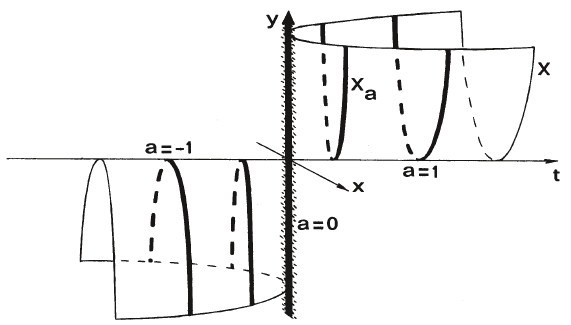
\includegraphics[scale=0.5]{3-3-1}
\end{figure}

Pero desde el punto de vista esquemático, $X_0=\spec(k[x,y]/\gene{x^2})$ nos da que la recta donde degeneran las parábolas es doble por los elementos nilpotentes. 
\end{ej}

\begin{ej}
De forma similar, si $X=\spec(k[x,y,t]/\gene{xy-t})$, obtenemos una familia cuyo miembto general $X_a$ es una hipérbola irreducible $xy=a$ cuando $a\neq 0$, pero cuyo miembro especial $X_0$ es el esquema reducible $xy=0$ consistente en dos rectas.
\end{ej}


\section{Ecualizador y coecualizador}
PENSAR SI PONER ESTO EN OTRA parte DEPENDIENDO DE LO QUE VEAMOS DESPUÉS

Sea $\CC$ una categoría y sean $f,g:X\to Y$ morfismos. Se dice que $e:Eq\to X$ satisfaciendo $f\circ eq= f\circ eq$ es un \emph{ecualizador} si para todo $m:Z\to X$ con $f \circ m=g\circ m$ existe un único $u:Z\to E$ tal que $eq\circ u=m$
\[
\begin{tikzcd}
E\arrow[r, "eq"] & X\arrow[r, shift left, "f"]\arrow[r, shift right, "g"'] & Y\\
Z\arrow[u, dashed, "u"]\arrow[ur, "m"] & 
\end{tikzcd}
\] 

\begin{ej}
En la categoría de conjuntos, dadas $\alpha, \alpha': A\to B$, el equalizador es el subconjunto $Eq(\alpha,\alpha')=\{a\in A\mid \alpha(a)=\alpha'(a')\}$. 
\end{ej}
Obsérvese que en una categoría aditiva, donde podemos sumar y restar morfismos, $Eq(\alpha,\alpha')=\ker(\alpha-\alpha')$. Dualmente se define el \emph{coecualizador} $Coeq$ mediante el siguiente diagrama
\[
\begin{tikzcd}
X\arrow[r, shift left, "f"]\arrow[r, shift right, "g"'] & Y\arrow[r, "q"] \arrow[dr, "q'"]& Coeq\arrow[d,dashed, "u"]\\
& & Z
\end{tikzcd}
\]
El coecualizador verifica la relación análoga con el conúcleo.
\begin{ej}
El coecualizador en la categoría de conjuntos, el coecualizador es el cociente $B/\sim$, donde $\sim$ es la relación generada por $\alpha(x)\sim\alpha'(x)$. 
\end{ej}
\begin{ej}
En $\mathrm{Top}$ tenemos los mismos ecualizadores y coecualizadores con las topologías inducidas correspondientes. 
\end{ej}

Sea $X=\bigcup_{i\in I}U_i$ un recubrimiento abierto del espacio $X$ y consideremos el coproducto $\coprod_{i\in I}U_i$. Tenemos el siguiente diagrama conmutativo 
\[
\begin{tikzcd}
\coprod_{(i,j)\in I^2}\in U_i\cap U_j\arrow[r, shift left, "\alpha"]\arrow[r, shift right,"\alpha'"']&\coprod_{i\in I}U_i\arrow[r, "\sigma"] & X\\
&U_i\arrow[u]\arrow[ur,hookrightarrow]&
\end{tikzcd}
\]
donde $\alpha$ es la inclusión con respecto al índice $i$ y $\alpha'$ con respecto al índice $j$. Se tiene entonces que $X=Coeq(\alpha,\alpha')$. Tenemos que probar que para todo espacio topológico $Z$ y para todo $h:\coprod U_i\to Z$ tal que $h\circ\alpha=h\circ\alpha'$, existe un único $\tilde{h}: X\to Z$ tal que $\tilde{h}\circ\sigma=h$. La aplicación $h$ está determinada por cada $h_i:U_i\to Z$, por lo que $h\circ \alpha=h\circ\alpha'$ si y solo si $h_i|_{U_i\cap U_j}=h_j|_{U_i\cap U_j}$, luego definimos $\tilde{h}$ pegando las $h_i$, que se pegan con continuidad porque coinciden en las intersecciones.

\begin{nota}
La condición de haz se puede expresar en una categoría más general (como la de conjuntos) como que $\calF(U)\to\prod_{i\in I}\calF(U_i\rightrightarrows \prod_{(i,j)}\calF(U_i\cap U_j)$ es un ecualizador, lo cual en cierto sentido se puede ver como una sucesión exacta. Además esto proviene del coecualizador $\coprod U_i\cap U_j\rightrightarrows \coprod U_i\to U$. En abiertos de un espacio $X$ se tiene además que $U_i\cap U_j$ es el producto fibrado $U_i\times_X U_j$. Con esto se consigue que si $F(X)=\Hom_{Top}(X,Z)$, entonces $F(X)\to \Hom_{Top}(\coprod X_i, Z)=\prod\Hom_{Top}(X_i,Z)\rightrightarrows \prod\Hom_{Top}(X_i\cap X_j,Z)$
\end{nota}

\begin{defi}[Topología de Grothendieck sobre una categoría]
Una topología en $\CC$ es una familia $Cov=\{X_i\to X\}_{i\in I}$ tal que
\begin{enumerate}
\item $\{Id:X\to X\}\in Cov$
\item  Si $\{X_i\to X\}, \{X_{ij}\to X_i\}\in Cov$, entonces $\{X_{ij}\to X\}\in Cov$.
\item Si $\{X_i\to X\}\in Cov$ y $Y\to X$, entonces $\{X_i\times_X Y\to Y\}\in Cov$. 
\end{enumerate} 
\end{defi}
Ejemplo de esto serían todas las familias de recubrimientos abiertos, ya sean de espacios topológicos sin más o esquemas (que sabemos que forman una categoría). Utilizando esta definición podemos definir haces sobre categorías. Un caso concreto muy importante es la topología \emph{Étale} sobre $\mathrm{Sch}_S$, donde las flechas de la definición tienen que ser morfismos étale:
\begin{defi}
Sabemos que para $f:A\to B$ y pra cualquier anillo $A\to C$ con un ideal $N^2=0$, tenemos el diagrama conmutativo
\[
\begin{tikzcd}
B \arrow[r, "\beta"] & C/N\\
A\arrow[u, "f"]\arrow[r, "\alpha"] & C\arrow[u, "\pi"]
\end{tikzcd}
\]
Decimos que $f$ es \emph{étale} si existe un único $\tilde{\beta}:B\to C$ que haga conmutar el diagrama. 
\end{defi}


\section{Ejercicios}
\begin{ejer}
Probar que el haz $\OO_X(U)$ es realmente un haz, describiendo las restricciones. 
\end{ejer}
\begin{ejer}
Probar que el prehaz $\calF(U)=\prod_{x\in U} A_x$ es un haz para $X$ con la topología discreta. 
\end{ejer}
\begin{ejer}
Probar el lema de Yoneda. 
\end{ejer}
\begin{ejer}
Consideramos $\Z[\frac{1}{2}]\hookrightarrow\Z[\frac{1}{2},i]$ (recordemos que 2 era el punto que daba problemas en la construcción del producto fibrado). Sea $C$ un anillo y $N$ un ideal tal que $N^2=0$. Supongamos que tenemos un diagramas conmutativos
\[
\begin{tikzcd}
\Z[i]\arrow[r, "\beta"] & C/N & & \Z[\frac{1}{2},i]\arrow[r] & C/N\\
\Z\arrow[u, hookrightarrow]\arrow[r, "\alpha"] & C\arrow[u, "p"'] & & \Z[\frac{1}{2}]\arrow[u]\arrow[r] & C\arrow[u]
\end{tikzcd}
\]
Comprobar que no siempre es posible levantar conmutativamente $\beta$ a $\Z[i]\to C$ pero siempre se puede hacer de manera única en el diagrama de la derecha con $\Z[\frac{1}{2},i]\to C$. Observar que $\alpha$ ya nos da a dónde tiene que ir $\Z$ luego tenemos que enviar $i$ a algo que respete $i^2+1=0$. Este ejercicio es equivalente a probar que $\Z\to\Z[i]$ no es étale pero $\Z[1/2]\to \Z[i,1/2]$ sí. 
\end{ejer}

\end{document}

